\documentclass[14pt,russian]{extarticle}		
\let\counterwithout\relax
\let\counterwithin\relax
\usepackage{lmodern}
\usepackage{float}
\usepackage{xcolor}
\usepackage{subfig}
\usepackage[export]{adjustbox}

\usepackage{setspace}
\onehalfspacing % полуторный интервал

%%%%%%%%%%%%%%%%%%%%%%%
%%% Проверка используемого TeX-движка %%%
\usepackage{iftex}
\newif\ifxetexorluatex   % определяем новый условный оператор (http://tex.stackexchange.com/a/47579/79756)
\ifXeTeX
    \xetexorluatextrue
\else
    \ifLuaTeX
        \xetexorluatextrue
    \else
        \xetexorluatexfalse
    \fi
\fi

%%% Поля и разметка страницы %%%
\usepackage{pdflscape}                              % Для включения альбомных страниц
\usepackage{geometry}                               % Для последующего задания полей
\geometry{a4paper,tmargin=2cm,bmargin=2cm,lmargin=3cm,rmargin=1cm} % тоже самое, но лучше

%%% Математические пакеты %%%
\usepackage{amsthm,amsfonts,amsmath,amssymb,amscd}  % Математические дополнения от AMS
\usepackage{mathtools}                              % Добавляет окружение multlined

%%%% Установки для размера шрифта 14 pt %%%%
%% Формирование переменных и констант для сравнения (один раз для всех подключаемых файлов)%%
%% должно располагаться до вызова пакета fontspec или polyglossia, потому что они сбивают его работу
\newlength{\curtextsize}
\newlength{\bigtextsize}
\setlength{\bigtextsize}{13.9pt}

\makeatletter
%\show\f@size                                       % неплохо для отслеживания, но вызывает стопорение процесса, если документ компилируется без команды  -interaction=nonstopmode 
\setlength{\curtextsize}{\f@size pt}
\makeatother

%%% Кодировки и шрифты %%%
\ifxetexorluatex
    \usepackage{polyglossia}                        % Поддержка многоязычности (fontspec подгружается автоматически)
\else
    \RequirePDFTeX                                  % tests for PDFTEX use and throws an error if a different engine is being used
   %%% Решение проблемы копирования текста в буфер кракозябрами
%    \input glyphtounicode.tex
%    \input glyphtounicode-cmr.tex %from pdfx package
%    \pdfgentounicode=1
    \usepackage{cmap}                               % Улучшенный поиск русских слов в полученном pdf-файле
    \defaulthyphenchar=127                          % Если стоит до fontenc, то переносы не впишутся в выделяемый текст при копировании его в буфер обмена
    \usepackage[T2A]{fontenc}                       % Поддержка русских букв
    \usepackage[utf8]{inputenc}                     % Кодировка utf8
    \usepackage[english, russian]{babel}            % Языки: русский, английский
    \IfFileExists{pscyr.sty}{\usepackage{pscyr}}{}  % Красивые русские шрифты
\fi

%%% Оформление абзацев %%%
\usepackage{indentfirst}                            % Красная строка

%%% Таблицы %%%
\usepackage{longtable}                              % Длинные таблицы
\usepackage{multirow,makecell,array}                % Улучшенное форматирование таблиц
\usepackage{booktabs}                               % Возможность оформления таблиц в классическом книжном стиле (при правильном использовании не противоречит ГОСТ)

%%% Общее форматирование
\usepackage{soulutf8}                               % Поддержка переносоустойчивых подчёркиваний и зачёркиваний
\usepackage{icomma}                                 % Запятая в десятичных дробях


%%% Гиперссылки %%%
\usepackage{hyperref}

%%% Изображения %%%
\usepackage{graphicx}                               % Подключаем пакет работы с графикой

%%% Списки %%%
\usepackage{enumitem}

%%% Подписи %%%
\usepackage{caption}                                % Для управления подписями (рисунков и таблиц) % Может управлять номерами рисунков и таблиц с caption %Иногда может управлять заголовками в списках рисунков и таблиц
\DeclareCaptionLabelFormat{continued}{Продолжение таблицы~#2.}
%% Использование:
%\begin{table}[h!]\ContinuedFloat - чтобы не переключать счетчик
%\captionsetup{labelformat=continued}% должен стоять до самого caption
%\caption{}
% либо ручками \caption*{Продолжение таблицы~\ref{...}.} :)

%%% Интервалы %%%

%%% Счётчики %%%
\usepackage[figure,table]{totalcount}               % Счётчик рисунков и таблиц
\usepackage{totcount}                               % Пакет создания счётчиков на основе последнего номера подсчитываемого элемента (может требовать дважды компилировать документ)
\usepackage{totpages}                               % Счётчик страниц, совместимый с hyperref (ссылается на номер последней страницы). Желательно ставить последним пакетом в преамбуле

%%% Продвинутое управление групповыми ссылками (пока только формулами) %%%
\ifxetexorluatex
    \usepackage{cleveref}                           % cleveref корректно считывает язык из настроек polyglossia
\else
    \usepackage[russian]{cleveref}                  % cleveref имеет сложности со считыванием языка из babel. Такое решение русификации вывода выбрано вместо определения в documentclass из опасности что-то лишнее передать во все остальные пакеты, включая библиографию.
\fi
\creflabelformat{equation}{#2#1#3}                  % Формат по умолч  
%%% Кодировки и шрифты %%%
\ifxetexorluatex
    \setmainlanguage[babelshorthands=true]{russian}  % Язык по-умолчанию русский с поддержкой приятных команд пакета babel
    \setotherlanguage{english}                       % Дополнительный язык = английский (в американской вариации по-умолчанию)
    \ifXeTeX
        \defaultfontfeatures{Ligatures=TeX,Mapping=tex-text}
    \else
        \defaultfontfeatures{Ligatures=TeX}
    \fi
	\setmainfont{Times New Roman}
	\newfontfamily\cyrillicfont{Times New Roman}
	\setsansfont{Times New Roman}                    %% задаёт шрифт без засечек
	\setmonofont{Liberation Mono}               %% задаёт моноширинный шрифт
\else
    \IfFileExists{pscyr.sty}{\renewcommand{\rmdefault}{ftm}}{}
\fi

%%% Интервалы %%%
%linespread-реализация ближе к реализации полуторного интервала в ворде.
%setspace реализация заточена под шрифты 10, 11, 12pt, под остальные кегли хуже, но всё же ближе к типографской классике. 
%\linespread{1.3}                    % Полуторный интервал (ГОСТ Р 7.0.11-2011, 5.3.6)

%%% Выравнивание и переносы %%%
\sloppy                             % Избавляемся от переполнений
\clubpenalty=10000                  % Запрещаем разрыв страницы после первой строки абзаца
\widowpenalty=10000                 % Запрещаем разрыв страницы после последней строки абзаца

%%% Подписи %%%
\captionsetup{%
singlelinecheck=off,                % Многострочные подписи, например у таблиц
skip=2pt,                           % Вертикальная отбивка между подписью и содержимым рисунка или таблицы определяется ключом
justification=centering,            % Центрирование подписей, заданных командой \caption
}
%%%        Подключение пакетов                 %%%
\usepackage{ifthen}                 % добавляет ifthenelse
%%% Инициализирование переменных, не трогать!  %%%
\newcounter{intvl}
\newcounter{otstup}
\newcounter{contnumeq}
\newcounter{contnumfig}
\newcounter{contnumtab}
\newcounter{pgnum}
\newcounter{bibliosel}
\newcounter{chapstyle}
\newcounter{headingdelim}
\newcounter{headingalign}
\newcounter{headingsize}
\newcounter{tabcap}
\newcounter{tablaba}
\newcounter{tabtita}
%%%%%%%%%%%%%%%%%%%%%%%%%%%%%%%%%%%%%%%%%%%%%%%%%%

%%% Область упрощённого управления оформлением %%%

%% Интервал между заголовками и между заголовком и текстом
% Заголовки отделяют от текста сверху и снизу тремя интервалами (ГОСТ Р 7.0.11-2011, 5.3.5)
\setcounter{intvl}{3}               % Коэффициент кратности к размеру шрифта

%% Отступы у заголовков в тексте
\setcounter{otstup}{0}              % 0 --- без отступа; 1 --- абзацный отступ

%% Нумерация формул, таблиц и рисунков
\setcounter{contnumeq}{1}           % Нумерация формул: 0 --- пораздельно (во введении подряд, без номера раздела); 1 --- сквозная нумерация по всей диссертации
\setcounter{contnumfig}{1}          % Нумерация рисунков: 0 --- пораздельно (во введении подряд, без номера раздела); 1 --- сквозная нумерация по всей диссертации
\setcounter{contnumtab}{1}          % Нумерация таблиц: 0 --- пораздельно (во введении подряд, без номера раздела); 1 --- сквозная нумерация по всей диссертации

%% Оглавление
\setcounter{pgnum}{0}               % 0 --- номера страниц никак не обозначены; 1 --- Стр. над номерами страниц (дважды компилировать после изменения)

%% Библиография
\setcounter{bibliosel}{1}           % 0 --- встроенная реализация с загрузкой файла через движок bibtex8; 1 --- реализация пакетом biblatex через движок biber

%% Текст и форматирование заголовков
\setcounter{chapstyle}{1}           % 0 --- разделы только под номером; 1 --- разделы с названием "Глава" перед номером
\setcounter{headingdelim}{1}        % 0 --- номер отделен пропуском в 1em или \quad; 1 --- номера разделов и приложений отделены точкой с пробелом, подразделы пропуском без точки; 2 --- номера разделов, подразделов и приложений отделены точкой с пробелом.

%% Выравнивание заголовков в тексте
\setcounter{headingalign}{0}        % 0 --- по центру; 1 --- по левому краю

%% Размеры заголовков в тексте
\setcounter{headingsize}{0}         % 0 --- по ГОСТ, все всегда 14 пт; 1 --- пропорционально изменяющийся размер в зависимости от базового шрифта

%% Подпись таблиц
\setcounter{tabcap}{0}              % 0 --- по ГОСТ, номер таблицы и название разделены тире, выровнены по левому краю, при необходимости на нескольких строках; 1 --- подпись таблицы не по ГОСТ, на двух и более строках, дальнейшие настройки: 
%Выравнивание первой строки, с подписью и номером
\setcounter{tablaba}{2}             % 0 --- по левому краю; 1 --- по центру; 2 --- по правому краю
%Выравнивание строк с самим названием таблицы
\setcounter{tabtita}{1}             % 0 --- по левому краю; 1 --- по центру; 2 --- по правому краю

%%% Рисунки %%%
\DeclareCaptionLabelSeparator*{emdash}{~--- }             % (ГОСТ 2.105, 4.3.1)
\captionsetup[figure]{labelsep=emdash,font=onehalfspacing,position=bottom}

%%% Таблицы %%%
\ifthenelse{\equal{\thetabcap}{0}}{%
    \newcommand{\tabcapalign}{\raggedright}  % по левому краю страницы или аналога parbox
}

\ifthenelse{\equal{\thetablaba}{0} \AND \equal{\thetabcap}{1}}{%
    \newcommand{\tabcapalign}{\raggedright}  % по левому краю страницы или аналога parbox
}

\ifthenelse{\equal{\thetablaba}{1} \AND \equal{\thetabcap}{1}}{%
    \newcommand{\tabcapalign}{\centering}    % по центру страницы или аналога parbox
}

\ifthenelse{\equal{\thetablaba}{2} \AND \equal{\thetabcap}{1}}{%
    \newcommand{\tabcapalign}{\raggedleft}   % по правому краю страницы или аналога parbox
}

\ifthenelse{\equal{\thetabtita}{0} \AND \equal{\thetabcap}{1}}{%
    \newcommand{\tabtitalign}{\raggedright}  % по левому краю страницы или аналога parbox
}

\ifthenelse{\equal{\thetabtita}{1} \AND \equal{\thetabcap}{1}}{%
    \newcommand{\tabtitalign}{\centering}    % по центру страницы или аналога parbox
}

\ifthenelse{\equal{\thetabtita}{2} \AND \equal{\thetabcap}{1}}{%
    \newcommand{\tabtitalign}{\raggedleft}   % по правому краю страницы или аналога parbox
}

\DeclareCaptionFormat{tablenocaption}{\tabcapalign #1\strut}        % Наименование таблицы отсутствует
\ifthenelse{\equal{\thetabcap}{0}}{%
    \DeclareCaptionFormat{tablecaption}{\tabcapalign #1#2#3}
    \captionsetup[table]{labelsep=emdash}                       % тире как разделитель идентификатора с номером от наименования
}{%
    \DeclareCaptionFormat{tablecaption}{\tabcapalign #1#2\par%  % Идентификатор таблицы на отдельной строке
        \tabtitalign{#3}}                                       % Наименование таблицы строкой ниже
    \captionsetup[table]{labelsep=space}                        % пробельный разделитель идентификатора с номером от наименования
}
\captionsetup[table]{format=tablecaption,singlelinecheck=off,font=onehalfspacing,position=top,skip=0pt}  % многострочные наименования и прочее
\DeclareCaptionLabelFormat{continued}{Продолжение таблицы~#2}

%%% Подписи подрисунков %%%
\renewcommand{\thesubfigure}{\asbuk{subfigure}}           % Буквенные номера подрисунков
\captionsetup[subfigure]{font={normalsize},               % Шрифт подписи названий подрисунков (не отличается от основного)
    labelformat=brace,                                    % Формат обозначения подрисунка
    justification=centering,                              % Выключка подписей (форматирование), один из вариантов            
}
%\DeclareCaptionFont{font12pt}{\fontsize{12pt}{13pt}\selectfont} % объявляем шрифт 12pt для использования в подписях, тут же надо интерлиньяж объявлять, если не наследуется
%\captionsetup[subfigure]{font={font12pt}}                 % Шрифт подписи названий подрисунков (всегда 12pt)

%%% Настройки гиперссылок %%%
\ifLuaTeX
    \hypersetup{
        unicode,                % Unicode encoded PDF strings
    }
\fi

\definecolor{linkcolor}{rgb}{0.0,0,0}
\definecolor{citecolor}{rgb}{0,0.0,0}
\definecolor{urlcolor}{rgb}{0,0,0}

\hypersetup{
    linktocpage=true,           % ссылки с номера страницы в оглавлении, списке таблиц и списке рисунков
%    linktoc=all,                % both the section and page part are links
%    pdfpagelabels=false,        % set PDF page labels (true|false)
    plainpages=true,           % Forces page anchors to be named by the Arabic form  of the page number, rather than the formatted form
    colorlinks,                 % ссылки отображаются раскрашенным текстом, а не раскрашенным прямоугольником, вокруг текста
    linkcolor={linkcolor},      % цвет ссылок типа ref, eqref и подобных
    citecolor={citecolor},      % цвет ссылок-цитат
    urlcolor={urlcolor},        % цвет гиперссылок
    pdflang={ru},
}
\urlstyle{same}
%%% Шаблон %%%
\DeclareRobustCommand{\todo}{\textcolor{red}}       % решаем проблему превращения названия цвета в результате \MakeUppercase, http://tex.stackexchange.com/a/187930/79756 , \DeclareRobustCommand protects \todo from expanding inside \MakeUppercase
\setlength{\parindent}{2.5em}                       % Абзацный отступ. Должен быть одинаковым по всему тексту и равен пяти знакам (ГОСТ Р 7.0.11-2011, 5.3.7).

%%% Списки %%%
% Используем дефис для ненумерованных списков (ГОСТ 2.105-95, 4.1.7)
\renewcommand{\labelitemi}{\normalfont\bfseries{--}} 
\setlist{nosep,%                                    % Единый стиль для всех списков (пакет enumitem), без дополнительных интервалов.
    labelindent=\parindent,leftmargin=*%            % Каждый пункт, подпункт и перечисление записывают с абзацного отступа (ГОСТ 2.105-95, 4.1.8)
}
%%%%%%%%%%%%%%%%%%%%%%
\usepackage{xltxtra} % load xunicode

\usepackage{ragged2e}
\usepackage[explicit]{titlesec}
\usepackage{placeins}
\usepackage{xparse}

\usepackage{listings}
\usepackage{url} %пакеты расширений
\usepackage{algorithm, algorithmicx}
\usepackage[noend]{algpseudocode}
\usepackage{blkarray}
\usepackage{chngcntr}

  
\titleformat{name=\section,numberless}[block]{\normalfont\Large\bfseries\centering}{}{0em}{#1}
\titleformat{\section}[block]{\normalfont\Large\bfseries\raggedright}{}{0em}{\thesection\hspace{0.25em}#1}
\titleformat{\subsection}[block]{\normalfont\Large\bfseries\raggedright}{}{0em}{\thesubsection\hspace{0.25em}#1}

\let\Algorithm\algorithm
\renewcommand\algorithm[1][]{\Algorithm[#1]\setstretch{1.5}}

\usepackage{pifont}
\usepackage{calc}
\usepackage{suffix}
\usepackage{csquotes}
\DeclareQuoteStyle{russian}
    {\guillemotleft}{\guillemotright}[0.025em]
    {\quotedblbase}{\textquotedblleft}
\ExecuteQuoteOptions{style=russian}
\newcommand{\enq}[1]{\enquote{#1}}  
\newcommand{\eng}[1]{\begin{english}#1\end{english}}
% Подчиненные счетчики в окружениях http://old.kpfu.ru/journals/izv_vuz/arch/sample1251.tex
\newcounter{cTheorem} 
\newcounter{cDefinition}
\newcounter{cConsequent}
\newcounter{cExample}
\newcounter{cLemma}
\newcounter{cConjecture}
\newtheorem{Theorem}{Теорема}[cTheorem]
\newtheorem{Definition}{Определение}[cDefinition]
\newtheorem{Consequent}{Следствие}[cConsequent]
\newtheorem{Example}{Пример}[cExample]
\newtheorem{Lemma}{Лемма}[cLemma]
\newtheorem{Conjecture}{Гипотеза}[cConjecture]

\renewcommand{\theTheorem}{\arabic{Theorem}}
\renewcommand{\theDefinition}{\arabic{Definition}}
\renewcommand{\theConsequent}{\arabic{Consequent}}
\renewcommand{\theExample}{\arabic{Example}}
\renewcommand{\theLemma}{\arabic{Lemma}}
\renewcommand{\theConjecture}{\arabic{Conjecture}}
%\makeatletter
\NewDocumentCommand{\Newline}{}{\text{\\}}
\newcommand{\sequence}[2]{\ensuremath \left(#1,\ \dots,\ #2\right)}

\definecolor{mygreen}{rgb}{0,0.6,0}
\definecolor{mygray}{rgb}{0.5,0.5,0.5}
\definecolor{mymauve}{rgb}{0.58,0,0.82}
\renewcommand{\listalgorithmname}{Список алгоритмов}
\floatname{algorithm}{Листинг}
\renewcommand{\lstlistingname}{Листинг}
\renewcommand{\thealgorithm}{\arabic{algorithm}}

\newcommand{\refAlgo}[1]{(листинг \ref{#1})}
\newcommand{\refImage}[1]{(рисунок \ref{#1})}

\renewcommand{\theenumi}{\arabic{enumi}.}% Меняем везде перечисления на цифра.цифра	
\renewcommand{\labelenumi}{\arabic{enumi}.}% Меняем везде перечисления на цифра.цифра
\renewcommand{\theenumii}{\arabic{enumii}.}% Меняем везде перечисления на цифра.цифра
\renewcommand{\labelenumii}{\arabic{enumi}.\arabic{enumii}.}% Меняем везде перечисления на цифра.цифра
\renewcommand{\theenumiii}{\arabic{enumiii}.}% Меняем везде перечисления на цифра.цифра
\renewcommand{\labelenumiii}{\arabic{enumi}.\arabic{enumii}.\arabic{enumiii}.}% Меняем везде перечисления на цифра.цифра
\newfontfamily\AnkaCoder[Path=src/fonts/]{AnkaCoder-r.ttf}
\renewcommand{\labelitemi}{--}
\renewcommand{\labelitemii}{--}

\makeatletter
\def\p@subsection{}
\def\p@subsubsection{\thesection\,\thesubsection\,}
\makeatother
\lstset{ %
  backgroundcolor=\color{white},   % choose the background color; you must add \usepackage{color} or \usepackage{xcolor}
  basicstyle=\footnotesize\AnkaCoder,        % the size of the fonts that are used for the code
  breakatwhitespace=false,         % sets if automatic breaks shoulbd only happen at whitespace
  breaklines=true,                 % sets automatic line breaking
  captionpos=top,                    % sets the caption-position to bottom
  commentstyle=\color{mygreen},    % comment style
  deletekeywords={...},            % if you want to delete keywords from the given language
  escapeinside={\%*}{*)},          % if you want to add LaTeX within your code
  extendedchars=true,              % lets you use non-ASCII characters; for 8-bits encodings only, does not work with UTF-8
  frame=single,                    % adds a frame around the code
  keepspaces=true,                 % keeps spaces in text, useful for keeping indentation of code (possibly needs columns=flexible)
  keywordstyle=\color{blue},       % keyword style
  language=python,                      % the language of the code
  morekeywords={uint64_t, uint8_t, int8_t,std,vector,uint32_t,Matrix,public,class,*,...},            % if you want to add more keywords to the set
  numbers=left,                    % where to put the line-numbers; possible values are (none, left, right)
  numbersep=5pt,                   % how far the line-numbers are from the code
  xleftmargin=25pt,
  xrightmargin=25pt,
  numberstyle=\small\color{mygray}, % the style that is used for the line-numbers
  rulecolor=\color{black},         % if not set, the frame-color may be changed on line-breaks within not-black text (e.g. comments (green here))
  showspaces=false,                % show spaces everywhere adding particular underscores; it overrides 'showstringspaces'
  showstringspaces=false,          % underline spaces within strings only
  showtabs=false,                  % show tabs within strings adding particular underscores
  stepnumber=1,                    % the step between two line-numbers. If it's 1, each line will be numbered
  stringstyle=\color{mymauve},     % string literal style
  tabsize=8,                       % sets default tabsize to 8 spaces
  title=\lstname                   % show the filename of files included with \lstinputlisting; also try caption instead of title
}
\newcommand{\anonsection}[1]{\cleardoublepage
\phantomsection
\addcontentsline{toc}{section}{\protect\numberline{}#1}
\section*{#1}}
\newcommand{\sectionbreak}{\clearpage}
\makeatletter
\let\@@scshape=\scshape
\renewcommand{\scshape}{%
  \ifnum\strcmp{\f@series}{bx}=\z@
    \usefont{T1}{cmr}{bx}{sc}%
  \else
    \ifnum\strcmp{\f@shape}{it}=\z@
      \fontshape{scsl}\selectfont
    \else
      \@@scshape
    \fi
  \fi}
\makeatother

\usepackage{caption} 
%\captionsetup[table]{justification=raggedleft} 
%\captionsetup[figure]{justification=centering,labelsep=endash}
\usepackage{amsmath}    % \bar    (матрицы и проч. ...)
\usepackage{amsfonts}   % \mathbb (символ для множества действительных чисел и проч. ...)
\usepackage{mathtools}  % \abs, \norm
    \DeclarePairedDelimiter\abs{\lvert}{\rvert}
    \DeclarePairedDelimiter\norm{\lVert}{\rVert}
\begin{document}
\sloppy

\def\figurename{Рисунок}

\begin{titlepage}
\thispagestyle{empty}
\newpage

\centerline{Министерство образования и науки РФ}
\centerline{Федеральное государственное бюджетное образовательное учреждение }
\centerline{Высшего профессионального образования}
\medskip 
\medskip 
\medskip
\centerline{Московский государственный технический университет имени Н.Э. Баумана}
 
\vspace{8em}
 
\begin{center}
\Large Расчетно-пояснительная записка к курсовому проекту по курсу \enq{Численные методы} \\
\end{center}
 
\begin{center}
\textsc{\textbf{Разработка электронного методического пособия для решения обыкновенных дифференциальных уравнений.}}
\end{center}
 
\vspace{\fill}
 

\newlength{\ML}
\settowidth{\ML}{«\underline{\hspace{0.7cm}}» \underline{\hspace{2cm}}}

\hfill\begin{minipage}{0.7\textwidth}
  Студент группы ИУ9-72\\
  \underline{\hspace{\ML}} Разборщикова~Анастасия Викторовна\\
  «\underline{\hspace{0.7cm}}» \underline{\hspace{2cm}} 2018 г.
\end{minipage}%
\bigskip

\hfill\begin{minipage}{0.7\textwidth}
  Преподаватель\\
  \underline{\hspace{\ML}} Домрачева~Анна Борисовна\\
  «\underline{\hspace{0.7cm}}» \underline{\hspace{2cm}} 2018 г.
\end{minipage}%
\vfill

%\vspace{\fill}
 


\begin{center}
Москва \\2018
\end{center}
\end{titlepage}
\newpage
\setcounter{page}{2}
\renewcommand\contentsname{Оглавление}
\tableofcontents
\newpage
\anonsection{Введение}    
	На сегодняшний день видна тенденция по автоматизации многих процессов, в том числе образовательных. Появляются новые методы и технологии обучения: удаленный доступ к лекционным материалам, автоматические системы тестирования и т.д. В связи с этим разрабатываются различные образовательные платформы, которые имеют свои плюсы и минусы. В интернете можно найти много приложений и онлайн-тренажеров для обучения, например, иностранным языкам, программированию, вождению.
	
	Однако фундаментальные дисциплины, как правило, все еще преподаются классическим методом: преподаватель читает лекционный материал, на семинарских занятиях разбираются некоторые задачи, часть задач остается студенту для самостоятельного разбора. При этом часто студент не имеет возможности проверить самостоятельно правильность своего решения до момента проверки преподавателем. В частности, такая проблема возникает при решении дифференциальных уравнений.
    
    В связи с этим необходимо произвести анализ существующих на данный момент систем тестирования, выявить существующие недостатки и создать приложение, восполняющие их. Например, предоставить возможность отработать решение определенного типа уравнений при помощи автоматической проверки ответа без использования тяжеловесных и дорогостоящих систем символьных вычислений или интернета.
    
    В данной работе поставлена задача реализовать инструмент для решения задачи Коши для обыкновенных дифференциальных уравнений (ОДУ) численными методами.
    
\section{Необходимые теоретические сведения}

Здесь и далее в определениях и формулах $t$ (либо $x$) --- независимая переменная, $y=y(t)$ --- зависимая переменная (искомая функция).

\begin{Definition}
\textit{Вычислительные методы} (\textit{численные методы} ) --- методы, используемые в вычислительной математике для преобразования вычислительных задач к виду, удобному для реализации на ЭВМ.~\cite[c.~55]{cite:Amosov}
\end{Definition}

\begin{Definition}
\textit{Вычислительная задача} --- одна из трех задач, возникающих при рассмотрении математических моделей:  прямая задача, обратная задача или задача идентификации \mbox{(см.~\cite[c.~43]{cite:Amosov}).}
\end{Definition}

\begin{Definition}
\textit{Решением} обыкновенного дифференциального уравнения первого порядка $y'=f(t, y(t)) $ называется дифференцируемая функция  $y(t)$, которая при подстановке в это уравнение обращает его в тождество. График решения дифференциального уравнения называют \textit{интегральной кривой}. Совокупность решений ДУ составляет \textit{поле направлений}. Для выделения \textit{частного решения} среди всего множества решений ДУ задают \textit{начальные условия} $y(t_0)=y_0$.~\cite[cc.~411-412]{cite:Amosov})
\end{Definition}

\begin{Definition}\label{def:Cauchy}
\textit{Задача Коши} (задача с начальными условиями) --- задача нахождения при $t > t_0$ решения дифференциального уравнения $y'=f(t, y(t)) $ при начальных условиях $y(t_0)=y_0$.~\mbox{\cite[c.~412]{cite:Amosov})}
\end{Definition}

Из теоремы существования и единственности (см.~\cite[c.~29]{cite:Filippov}) следует, что для существования решения задачи Коши, на отрезке достаточно непрерывности функции $f(t, y(t))$. Так как аналитически можно решить лишь некоторый класс известных типов дифференциальных уравнений (в то время как на самом деле решение имеет намного более широкий класс), вычислительные методы являются более универсальными, так как имеют, как правило, меньше ограничений по сравнению с аналитическими и часто позволяют найти приближенное решение там, где это невозможно сделать символьно.

\section{Обзор аналогов}
Рассмотрим несколько популярных обучающих платформ: Coursera, Udemy, Stepik, Intuit, MathSemester - выделим их общие элементы, плюсы и минусы. Так же проведем краткий обзор некоторых аналогов, доступных для платформы Android на момент написания данной работы.

\subsection{Coursera}

Платформа была основана в 2012 году Стэнфордскими профессорами в области компьютерных наук, которые хотели сделать свои знания доступными онлайн. Сейчас на сайте 35 млн студентов и более 2,700 курсов. Есть возможность получить степень магистра. Платформа содержит курсы от ведущих университетов и организаций. По завершении курса слушатель может получает сертификат.~\cite{cite:Coursera_about}

На сайте есть бесплатный курс обыкновенных дифференциальных уравнений от Корейского универстета передовых технологий (Korea Advanced Institute of Science and Technology). В программу курса включены видео с объяснениями преподавателя и практические упражнения (тесты). На момент написания работы этот курс -- единственный курс Coursera, посвященный дифференциальным уравнениям (поиск велся как на русском, так и на английском языках).

На рисунках~\ref{img:Coursera:1} и~\ref{img:Coursera:2} приведены скриншоты с примерами подачи теоретического материала и тестирования.

%\begin{figure}[h!]
%	\centering
%		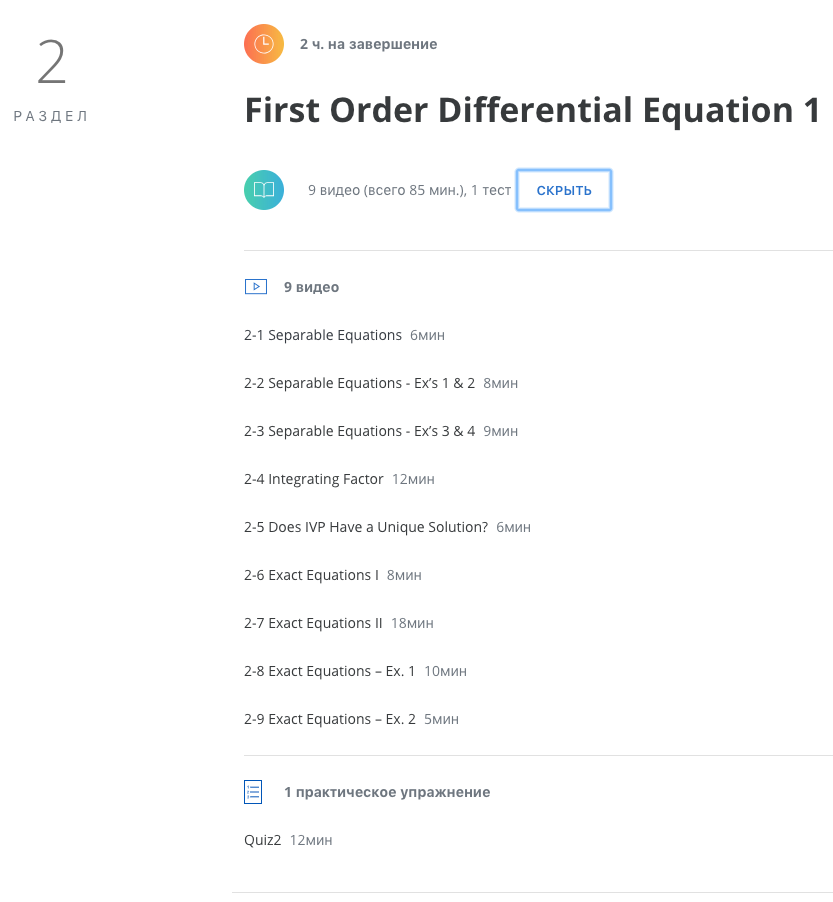
\includegraphics[height=12cm]{img/Coursera/pic1.png}
%	\caption{Программа курса дифференциальных уравнений от Корейского университета передовых технологий на платформе Coursera.}
%	\label{img:Coursera:1}
%\end{figure}

\begin{figure}[h!]
	\centering
		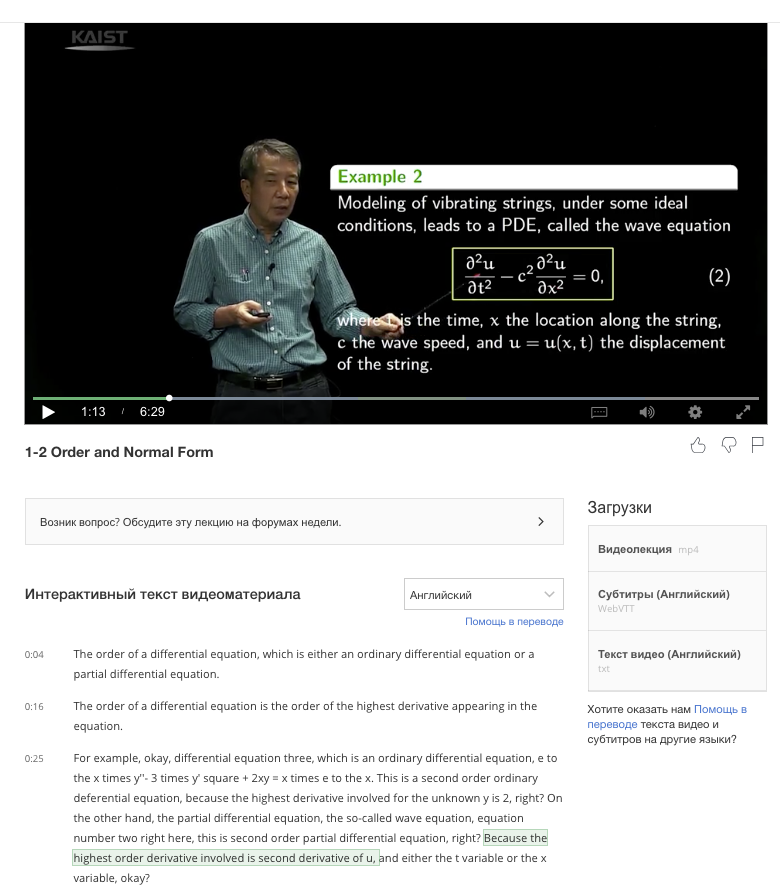
\includegraphics[height=.4\textheight]{img/Coursera/pic2.png}
	\caption{Формат изложения теоретического материала на платформе Coursera.}
	\label{img:Coursera:1}
\end{figure}

\begin{figure}[h!]
	\centering
		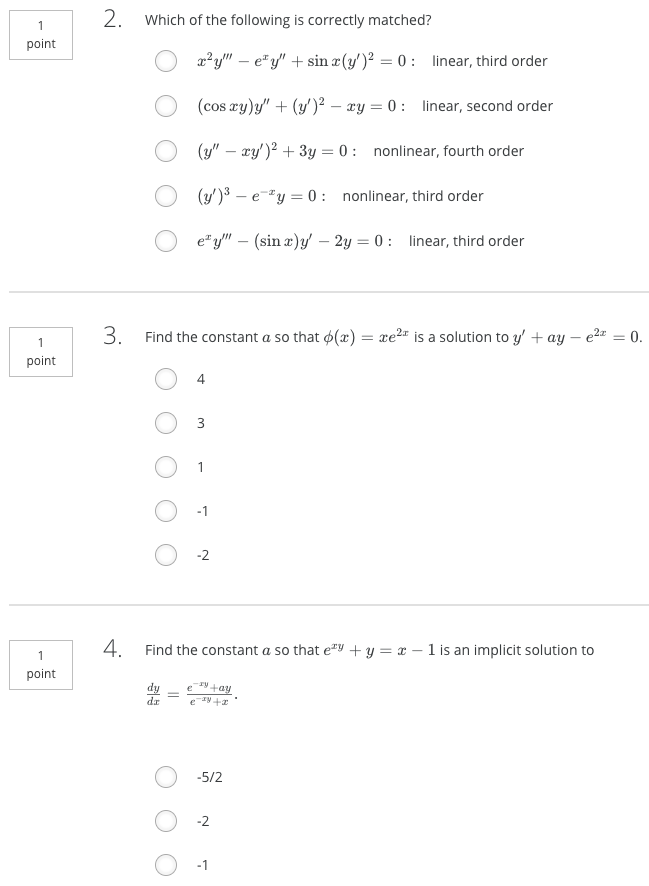
\includegraphics[height=.4\textheight]{img/Coursera/pic3.png}
	\caption{Пример тестирования по курсу дифференциальных уравнений на платформе Coursera.}
	\label{img:Coursera:2}
\end{figure}

%\begin{table}[h!]
%	\centering
%		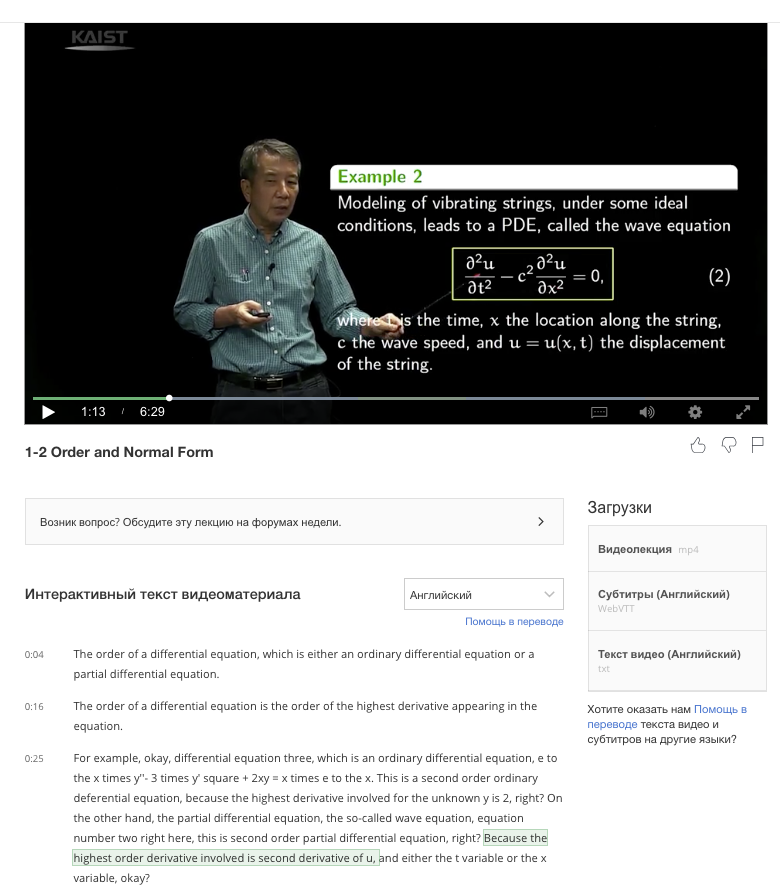
\includegraphics[width=0.5\linewidth]{img/Coursera/pic2.png}
%		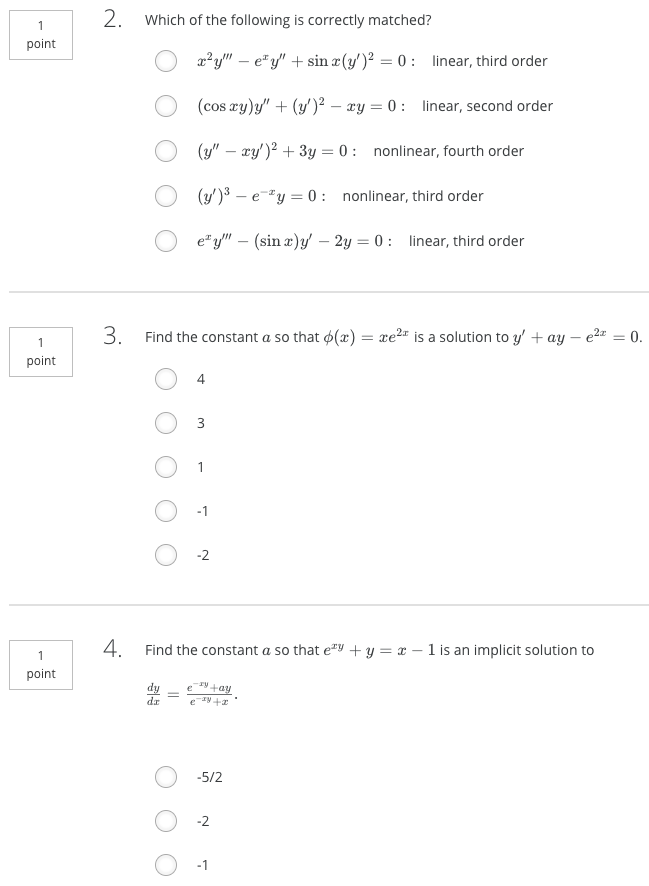
\includegraphics[width=0.5\linewidth]{img/Coursera/pic3.png}
%	\caption{Пример изложения теоретического материала (слева) и тестирования (справа) по курсу дифференциальных уравнений на платформе Coursera.}
%	\label{img:Coursera:2}
%\end{table}

%\begin{figure}%
%    \centering
%    \subfloat{{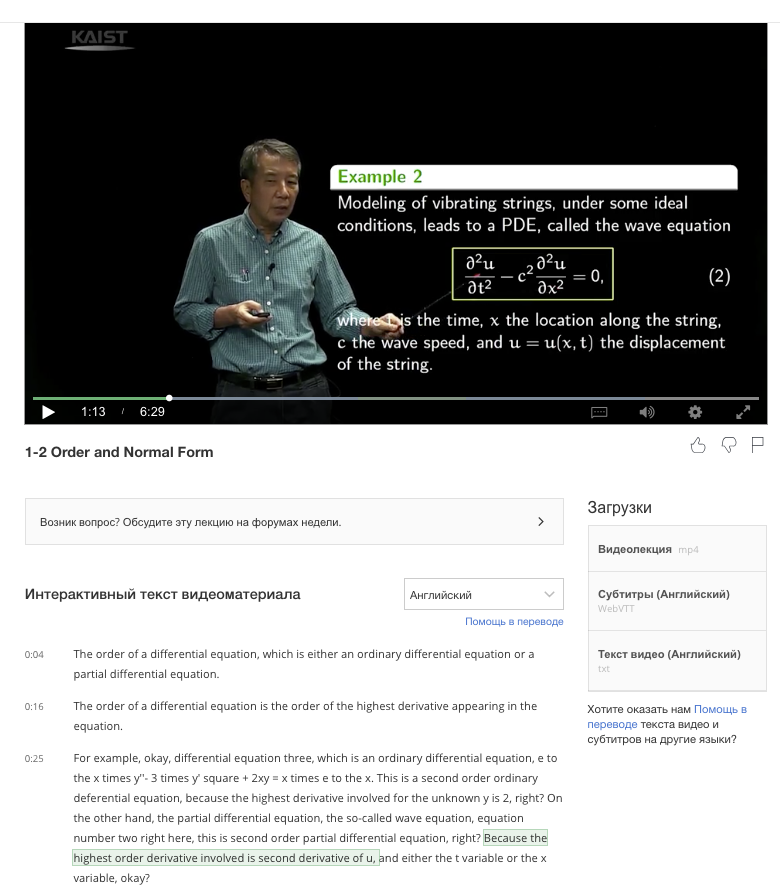
\includegraphics[width=.46\linewidth]{img/Coursera/pic2.png} }}%
%    \qquad
%    \subfloat{{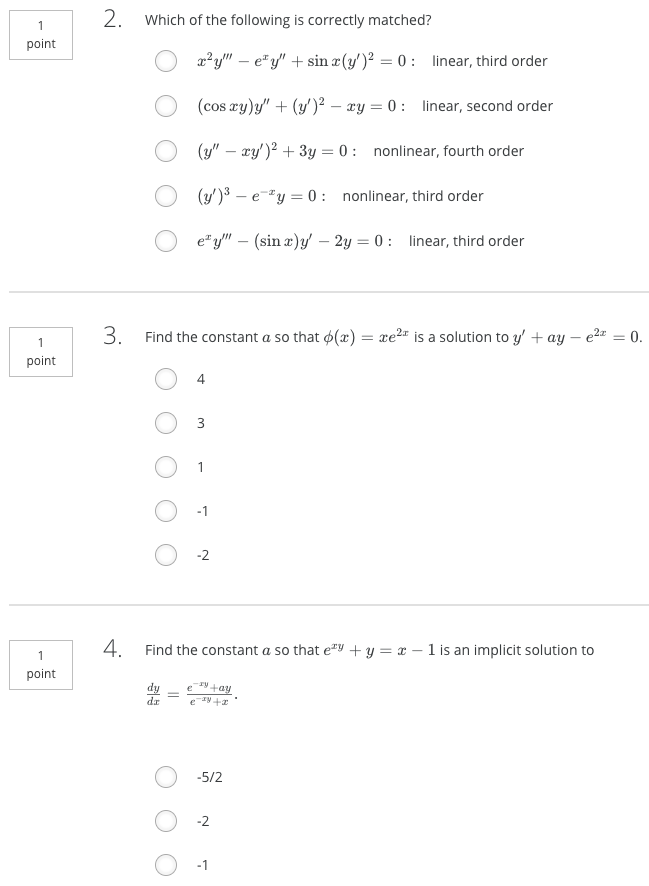
\includegraphics[width=.46\linewidth]{img/Coursera/pic3.png} }}%
%    \caption{Пример изложения теоретического материала (слева) и тестирования (справа) по курсу дифференциальных уравнений на платформе Coursera.}%
%    \label{img:Coursera:2}%
%\end{figure}


\subsection{Udemy}

Данная платформа, в отличие от Coursera, не является академической, то есть курсы, представленные на ней, не аккредитованы высшими университетами, институтами или колледжами. В основном курсы рассчитаны на работающих взрослых, которые хотят улучшить свои профессиональные навыки, а так же компании, желающие расширить компетенции своих сотрудников. Многие курсы являются платными и приносят доход своим авторам. Платформа позволяет добавлять в курс видео, PowerPoint-презентации, PDF-файлы, аудио, файловые архивы, чаты. По заявлению создателей, Udemy является лидирующей площадкой для обучения и объединения студентов. На данный момент она предоставляет около 100 тыс. курсов от 42 тыс. инструкторов для 30 млн. обучающихся. По завершению курса слушателям предоставляются сертификаты.~\cite{cite:Udemy_about}

На момент написания работы на платформе представлено 7 курсов по запросу \enquote{differential equations} стоимостью от 19,99\$ до 89,99\$. Ни одного курса на русском языке найдено не было. Курсы предлагают видео-лекции и печатные материалы для скачивания.

\subsection{Национальный Открытый Университет «ИНТУИТ»}
ООО «Интуит.ру» -- некоммерческая организация, в 2016 году получившая лицензию Департамента образования города Москвы на предоставление дополнительного профессионального образования. Курсы на этой платформе создаются как организациями (академиями, университетами, коммерческими фирмами), так и частными авторами. По окончании курса слушатель может получить бесплатный электронный сертификат, также есть возможность получить платно сертификат о повышении квалификации. Есть возможность получить высшее образование дистанционно.~\cite{cite:Intuit_about}

 Помимо онлайн-курсов организация выпускает учебную литеру (книги, DVD), действуя, как издательство. Также существует приложение, предоставляющее доступ к возможностям платформы с мобильных устройств.

На момент написания работы платформа содержит три бесплатных курса на русском языке, посвященных дифференциальным уравнениям. Все они имеют одинаковое содержание: предоставляют записи лекций, размещенные на видеохостинге YouTube,
%~(рис.~\pageref{img:Intuit:1}.),
и тесты в формате, представленном на~рис.~\ref{img:Intuit:2}.

%\begin{figure}[h!]
%	\centering
%		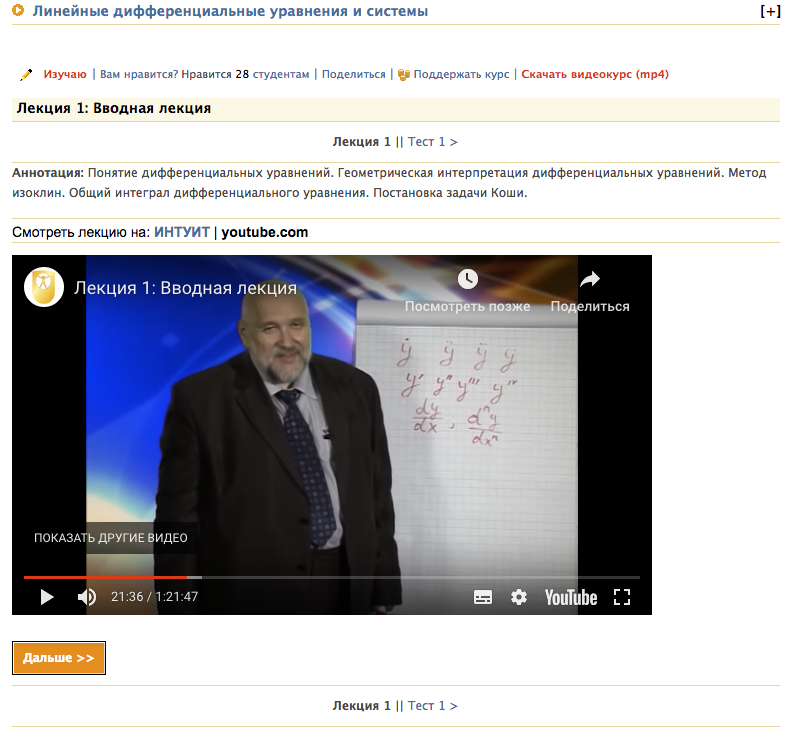
\includegraphics[height=.4\textheight]{img/Intuit/pic1.png}
%	\caption{Пример предоставления лекционного материала платформой \enquote{Интуит.ру}.}
%	\label{img:Intuit:1}
%\end{figure}

\begin{figure}[h!]
	\centering
		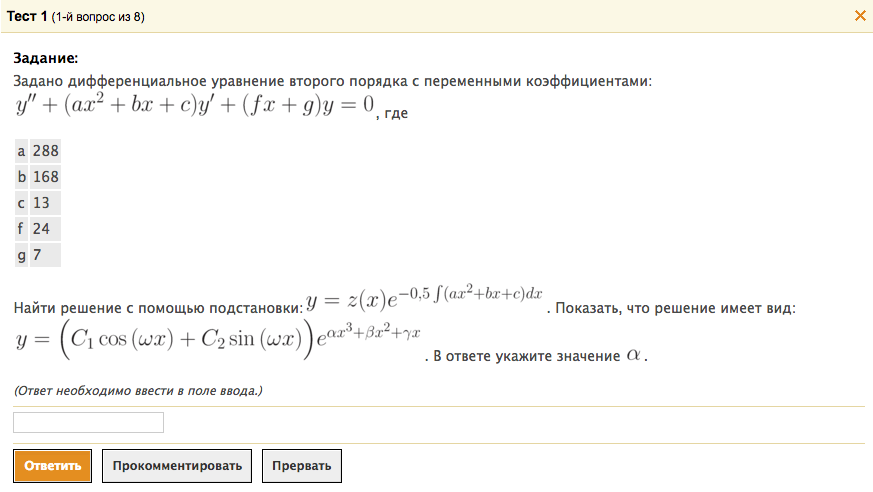
\includegraphics[height=.4\textheight]{img/Intuit/pic2.png}
	\caption{Пример теста для курса \enquote{Дифференциальные уравнения} на сайте \enquote{Интуит.ру}.}
	\label{img:Intuit:2}
\end{figure}

\subsection{Stepik}

\enquote{Первые учебные материалы были размещены на платформе в 2013 году. Сегодня среди охваченных курсами тем: программирование, информатика, математика, статистика 
и анализ данных, биология и биоинформатика, инженерно-технические и естественные науки. Онлайн-курсы, размещенные на Stepik, неоднократно становились призерами конкурсов онлайн-курсов, а система автоматизированной проверки задач используется 
в ряде курсов на платформах Coursera и edX. Также Stepik активно развивает направление адаптивного обучения, где каждый сможет изучать материал, подобранный индивидуально под свой уровень знаний.} (Цитата с сайта Stepic.org~\cite{cite:Stepik_about})

На момент написания работы платформа не содержит курсов по запросу \enquote{дифференциальные уравнения} или \enquote{differential equations}.

Для остальных курсов платформа предлагает учебный материал в виде слайдов, записей лекций. Контрольные задания выполняются в виде автоматизированных тестов и ответов в свободной форме, проверяемых преподавателем. Платформа имеет мобильное приложение с тем же функционалом.

\subsection{Сравнение платформ}
В завершение обзора проведем сравнение обозреваемых платформ в таблице~\ref{table:platform_comparison}. Стоит отметить, что, во-первых, все из перечисленных платформ предоставляют преимущественно теоретический материал. Наибольшую практическую направленность (больше типов заданий для проверки, вплоть до автоисполнения программного кода) имеет Stepik, в то время как Udemy вообще не имеет механизмов проверки знаний. Coursera и Intuit являются более академическими ресурсами, позволяющими получить не только сертификат об окончании курса, но и ученую степень (Coursera) или сертификат по повышении квалификации (Intuit).


\begin{table}[H]
\caption{Сравнение образовательных платформ.\label{table:platform_comparison}}
\begin{center}
\begin{tabular}{|c|c|c|c|c|}
\hline 
\multirow{4}{*}{Платформа}&Кто может            & Есть ли                    &    Теоретический  &   Практические \\
                                                 &создавать            & материалы              &  материал              &   упражнения     и       \\
                                                 &курсы                   & по теме ДУ              &                                 &   тесты  \\
\hline
\multirow{3}{*}{Coursera} & Универси-               &                                  &                                & Автомати-\\
                                            & теты и орга-            &Есть,      на               & Видео,                    & зированные и \\
                                            &        низации            & английском             &  слайды                   & проверяемые  \\
                                            &                                   &                                   &                                & учителем  \\                            
\hline
\multirow{4}{*}{Udemy}    &                            &                                        & Видео,                    & \\
                                            &  Любой               &                ---                  & аудио,                     &  --- \\
                                            &желающий         &                                        & PPT-презентации,& \\
                                            &                            &                                        &  PDF-файлы,          &\\
                                            &                            &                                        &  ZIP-архивы         &\\
\hline
\multirow{5}{*}{Intuit   }    &  Любой               &   3 бесплатных             & Видео на                  & Тесты\\
                                            &желающий         &       курса  на                 & видеохостинге     &  и вопросы \\
                                            &(аккредитация  &         русском                &  YouTube,              & с ответом в\\
                                            & Департамента  &       языке                      &  текст                    & свободной\\
                                            &образования)    &                                         &                               & форме\\
\hline
\multirow{4}{*}{Stepik}     &                            &                                        &                                  & Тесты, задачи,\\
                                            &  Любой               &                ---                  & Видео,                     &  проверяемые  \\
                                            &желающий         &                                        & текстовые             & учителем,\\
                                            &                            &                                        &  материалы          & Автотести-\\
                                            &                            &                                        &                                &рование кода\\
\hline
\end{tabular} 
\end{center}
\end{table}


Все из перечисленных систем имеют мобильные приложения, предоставляющие доступ к функционалу платформ с мобильных устройств.

Тестирующие модули рассмотренных обучающих систем разработаны только для контроля усвоения знаний и выставления прогресса обучающегося. Ни один из них не может быть использован для отработки навыков и самопроверки, что позволяет сделать вывод о необходимости разработки такого инструмента.

\subsection{Мобильные приложения для решения дифференциальных уравнений}

Для мобильных устройств (рассмотрим Andoid и официальных магазин приложений Play Store) существует несколько приложений, позволяющих решать дифференциальные уравнения численно.

Несмотря на то, что по запросам \enquote{differential equations} и \enquote{дифференциальные уравнения} было получено большое количество результатов, лишь несколько приложений соответствуют искомой тематике и позволяют решать дифференциальыне уравнения.

\begin{table}[H]
\caption{Сравнение мобильных приложений.\label{table:apps_comparison}}
\begin{center}
\begin{tabular}{|c|c|c|c|c|}
\hline 
Название                                    & Алгоритм           &  Формат &  \multirow{2}{*}{Преимущества}     & \multirow{2}{*}{Недостатки} \\
приложения                               &решения              & решения &&\\
\hline 
DE Solver Free                             &   Численный        & График             & Решение                   &  Нет  \\
(SunshineTechie)                        &                                 &     функции        &   уравнений  II       & решений \\
                                                      &                                &                            &  и III порядков       & систем ОДУ\\
\hline
Differential                                   &                               & Пошаговое           & Разбор                & Решение  \\
Equations Steps                          &    Символьный     &     решение           &   хода                  & доступно при \\
(Ivan Petuhov)                            &                                &                                &  решения            & подписке\\
\hline
Symbolab --                                   &                               & Аналитичес-& Аналитическое     & Нет \\
Math Solver                            &    Символьный     &   кое  решение&  решение                & решений  \\
(Symbolab)                            &                                &   и   график&                               & систем ОДУ\\
\hline

\end{tabular} 
\end{center}
\end{table}

Многие приложения с похожими названиями не подходят для решения обыкновенных дифференциальных уравнений. Например:
\begin{itemize}
\item Differential equations (referencehunt) содержит только теоретические сведения о решении дифференциальных уравнений;
\item PDE Solver дает возможность решать только уравнения в частных производных (в данной работе поставлена задача решения обыкновенных дифференциальных уравнений);
\item Equation Solver (Alex Gwyn) позволяет решать только алгебраические уравнения.
\end{itemize}

Таким образом, существующие решения имеют либо не предоставляют некоторый функционал, либо платны, в связи с чем возникает необходимость создания инструмента, покрывающего эти недостатки.

\section{Реализация приложения}

\subsection{Базовая концепция}
Для реализации системы самопроверки было выбрано автономное Android-приложение, так как оно позволит инструменту быть доступным и мобильным.

Для обеспечения автономности и высокой скорости работы и простоты реализации были выбраны численные методы решения дифференциальных уравнений. Вывод численного решения на экран пользователю предоставляется в виде графика функции (интегральной кривой).

В рамках данной работы была поставлена задача реализовать решение задачи Коши численными методами.

Согласно определению~\ref{def:Cauchy} (с.~\pageref{def:Cauchy}) и техническому заданию, интерфейс приложения должен обладать следующими базовыми элементами:
\begin{itemize}
\item поле для ввода уравнения $y'=f(x, y)$;
\item поля для ввода начальных условий $x_0$ и $y(x_0)$;
\item вывод графика решения;
\item возможность проверить решение пользователя.
\end{itemize}

Для проверки решения пользователя было решено выводить на одном графике полученные численно изоклины и график пользовательского решения.

Графическое представление решения ДУ позволяет судить о поведении функции и характере физического явления, описываемого данной задачей Коши.

\subsection{Алгоритмы}

Существуют различные численные методы решения задачи Коши~\mbox{\cite[cc.~410-481]{cite:Amosov}}. Они отличаются погрешностью, скоростью сходимости, устойчивостью.

\begin{Definition}
Решение $\bold{y} =\bold\varphi(t)$ системы дифференциальных уравнений \mbox{$\bold{y} = \bold f (t, \bold y)$}, \mbox{$\bold y = (y_1, \dots, y_n)$} называют устойчивым по Ляпунову (устойчивым), если для любого \mbox{$\varepsilon>0$} существует такое \mbox{$\delta > 0$}, что для всякого решения $\bold y(t)$ той же системы, начальное значение которого удовлетворяет неравенству
$$|y(t_0)-\varphi(t_0)| < \delta,$$
при всех $t \geq t_0$ выполняется неравенство
$$|y(t) < \varphi(t)| < \varepsilon.$$

Если же такого $\varepsilon > 0$ не существует, то решение $\varphi(t)$ называется неустойчивым.

Решение $\varphi(t)$ называется асимптотически устойчивым, если оно устойчиво по Ляпунову и, кроме того, все решения с достаточно близкими начальными условиями неограниченно приближаются к $\varphi(t)$ при $ t \rightarrow +\inf$, то есть если из неравенства $|y(t_0)-\varphi(t_0)| < \delta$ следует $y(t)-\varphi(t) \rightarrow 0$ \mbox{$(t\rightarrow +\inf)$}.

Наличие или отсутствие устойчивости не зависит от \mbox{выбора $t_0$.~\cite[cc.~87-88]{cite:Filippov}}
\end{Definition}

Выбор метода численного решения 
\subsection{Фреймворки и структуры данных}

\section{Тестирование}
\subsection{Интерфейс}
\subsection{Валидация}
\subsection{Обработка ошибок}


%
\anonsection{Заключение}


% Список литературы
\clearpage
\bibliographystyle{src/utf8gost705u}%gost2008} utf8gost705u}
{\catcode`"\active\def"{\relax}
\addcontentsline{toc}{section}{\protect\numberline{}\refname}%
\bibliography{biblio}
\end{document}
